\documentclass[,aspectratio=169]{beamer}

% Load theme ---------------------------------------------------------------------------------

\usetheme[transitions,banner,logo]{ubd}

% Information for the title page -------------------------------------------------------------
\author{Drs. Haziq Jamil \& Huda Ramli}

\title{SM-2302 Software for Mathematicians}

\title{SM-2302 Software for Mathematicians}

\subtitle{Introduction \& Getting Started}

\institute{Mathematical Sciences, Faculty of Science, UBD\\
\url{https://sm2302.github.io}}

\date{Semester I 2022/23}

% Font fix -----------------------------------------------------------------------------------
% \usepackage{ifxetex,ifluatex}
% \ifnum 0\ifxetex 1\fi\ifluatex 1\fi=0 % if pdftex
%   \usepackage[T1]{fontenc}
%   \usepackage[utf8]{inputenc}
%   \usepackage{textcomp} % provide euro and other symbols
% \else % if luatex or xetex
%   \usepackage{unicode-math}
%   \defaultfontfeatures{Scale=MatchLowercase}
%   \defaultfontfeatures[\rmfamily]{Ligatures=TeX,Scale=1}
% \fi

\usepackage{soul}
\makeatletter
\let\HL\hl
\renewcommand\hl{%
  \let\set@color\beamerorig@set@color
  \let\reset@color\beamerorig@reset@color
  \HL}
\makeatother
% https://tex.stackexchange.com/questions/460731/highlight-color-a-part-of-text-in-block-in-beamer
\newcommand{\hlc}[2][yellow]{{%
    \colorlet{foo}{#1}%
    \sethlcolor{foo}\hl{#2}}%
}
% https://tex.stackexchange.com/questions/352956/how-to-highlight-text-with-an-arbitrary-color

% knitr stuff --------------------------------------------------------------------------------
\usepackage{color}
\usepackage{fancyvrb}
\newcommand{\VerbBar}{|}
\newcommand{\VERB}{\Verb[commandchars=\\\{\}]}
\DefineVerbatimEnvironment{Highlighting}{Verbatim}{commandchars=\\\{\}}
% Add ',fontsize=\small' for more characters per line
\usepackage{framed}
\definecolor{shadecolor}{RGB}{248,248,248}
\newenvironment{Shaded}{\begin{snugshade}}{\end{snugshade}}
\newcommand{\AlertTok}[1]{\textcolor[rgb]{0.94,0.16,0.16}{#1}}
\newcommand{\AnnotationTok}[1]{\textcolor[rgb]{0.56,0.35,0.01}{\textbf{\textit{#1}}}}
\newcommand{\AttributeTok}[1]{\textcolor[rgb]{0.77,0.63,0.00}{#1}}
\newcommand{\BaseNTok}[1]{\textcolor[rgb]{0.00,0.00,0.81}{#1}}
\newcommand{\BuiltInTok}[1]{#1}
\newcommand{\CharTok}[1]{\textcolor[rgb]{0.31,0.60,0.02}{#1}}
\newcommand{\CommentTok}[1]{\textcolor[rgb]{0.56,0.35,0.01}{\textit{#1}}}
\newcommand{\CommentVarTok}[1]{\textcolor[rgb]{0.56,0.35,0.01}{\textbf{\textit{#1}}}}
\newcommand{\ConstantTok}[1]{\textcolor[rgb]{0.00,0.00,0.00}{#1}}
\newcommand{\ControlFlowTok}[1]{\textcolor[rgb]{0.13,0.29,0.53}{\textbf{#1}}}
\newcommand{\DataTypeTok}[1]{\textcolor[rgb]{0.13,0.29,0.53}{#1}}
\newcommand{\DecValTok}[1]{\textcolor[rgb]{0.00,0.00,0.81}{#1}}
\newcommand{\DocumentationTok}[1]{\textcolor[rgb]{0.56,0.35,0.01}{\textbf{\textit{#1}}}}
\newcommand{\ErrorTok}[1]{\textcolor[rgb]{0.64,0.00,0.00}{\textbf{#1}}}
\newcommand{\ExtensionTok}[1]{#1}
\newcommand{\FloatTok}[1]{\textcolor[rgb]{0.00,0.00,0.81}{#1}}
\newcommand{\FunctionTok}[1]{\textcolor[rgb]{0.00,0.00,0.00}{#1}}
\newcommand{\ImportTok}[1]{#1}
\newcommand{\InformationTok}[1]{\textcolor[rgb]{0.56,0.35,0.01}{\textbf{\textit{#1}}}}
\newcommand{\KeywordTok}[1]{\textcolor[rgb]{0.13,0.29,0.53}{\textbf{#1}}}
\newcommand{\NormalTok}[1]{#1}
\newcommand{\OperatorTok}[1]{\textcolor[rgb]{0.81,0.36,0.00}{\textbf{#1}}}
\newcommand{\OtherTok}[1]{\textcolor[rgb]{0.56,0.35,0.01}{#1}}
\newcommand{\PreprocessorTok}[1]{\textcolor[rgb]{0.56,0.35,0.01}{\textit{#1}}}
\newcommand{\RegionMarkerTok}[1]{#1}
\newcommand{\SpecialCharTok}[1]{\textcolor[rgb]{0.00,0.00,0.00}{#1}}
\newcommand{\SpecialStringTok}[1]{\textcolor[rgb]{0.31,0.60,0.02}{#1}}
\newcommand{\StringTok}[1]{\textcolor[rgb]{0.31,0.60,0.02}{#1}}
\newcommand{\VariableTok}[1]{\textcolor[rgb]{0.00,0.00,0.00}{#1}}
\newcommand{\VerbatimStringTok}[1]{\textcolor[rgb]{0.31,0.60,0.02}{#1}}
\newcommand{\WarningTok}[1]{\textcolor[rgb]{0.56,0.35,0.01}{\textbf{\textit{#1}}}}
\usepackage{graphicx,grffile}
\makeatletter
\def\maxwidth{\ifdim\Gin@nat@width>\linewidth\linewidth\else\Gin@nat@width\fi}
\def\maxheight{\ifdim\Gin@nat@height>\textheight\textheight\else\Gin@nat@height\fi}
\makeatother
% Scale images if necessary, so that they will not overflow the page
% margins by default, and it is still possible to overwrite the defaults
% using explicit options in \includegraphics[width, height, ...]{}
\setkeys{Gin}{width=\maxwidth,height=\maxheight,keepaspectratio}
% Set default figure placement to htbp
\makeatletter
\def\fps@figure{htbp}
\makeatother
\setlength{\emergencystretch}{3em} % prevent overfull lines
\providecommand{\tightlist}{%
  \setlength{\itemsep}{0pt}\setlength{\parskip}{0pt}}
\setcounter{secnumdepth}{-\maxdimen} % remove section numbering

% Reduce spacing between code and output knitr
\AtBeginEnvironment{verbatim}{\vspace{-2em}}



% Packages -----------------------------------------------------------------------------------
% \setlength{\parskip}{1em}
\usepackage{tikz}
\usetikzlibrary{shapes.geometric,fit,arrows.meta}
\usepackage{xltabular}
\usepackage{longtable,booktabs,multirow,colortbl}
\usepackage{caption}
% Make caption package work with longtable
\makeatletter
\def\fnum@table{\tablename~\thetable}
\makeatother
\usepackage{lipsum}
\usepackage{csquotes}

% To use arabic -----------------------------------------------------------------------------
% WARNING: Using arabic script causes some issues with footnotes.
% Packages are not loaded by default

\usepackage{polyglossia}  
% \setdefaultlanguage{english}
% \setotherlanguage{arabic} % to use arabic
% \newfontfamily\arabicfontsf[Script=Arabic]{Amiri}

% % Fix for footnotes not showing when arabic script used
% % https://tex.stackexchange.com/questions/228075/beamer-in-arabic-language-doesnt-accept-footnotes
% \makeatletter
% \let\@footnotetext=\beamer@framefootnotetext
% \makeatother

% % Fix for footnotes not showing when using \footnote<.->
% \let\oldfootnote\footnote
% \renewcommand{\footnote}{\only<+->\oldfootnote}
% % https://stackoverflow.com/questions/62345074/show-footnote-only-after-a-pause-in-beamer-with-r-markdown

% Fonts -----------------------------------------------------------------------------------
\usepackage{cmbright}
\usefonttheme{default}
\usepackage{pifont}% http://ctan.org/pkg/pifont
\newcommand{\cmark}{\ding{51}}%
\newcommand{\xmark}{\ding{55}}%

% Bibliography

% Fix URL, DOI, ISBN, etc. font in biblatex
% https://tex.stackexchange.com/questions/416093/change-font-of-the-word-url-before-the-actual-url-in-biblatex
% \renewcommand*{\mkbibacro}[1]{#1}  

\newcommand{\thankyou}{%
	{
		\begin{frame}[plain,noframenumbering]{End}
			\centering
			\Huge Thank you!
		\end{frame}
	}

}

% Maths -----------------------------------------------
\usepackage{empheq}
\newcommand*\mybox[1]{%
\colorbox{navyblue!35}{#1}}

\usepackage[skins,theorems]{tcolorbox}
\tcbset{highlight math style={enhanced,
  colframe=navyblue,colback=white,arc=2pt,boxrule=1pt}}

\usepackage{amssymb}
\usepackage{dsfont}  % for indicator variables \mathsds{1}
\usepackage{bm}  % for better bold script
\usepackage[makeroom]{cancel}
\usepackage{centernot}
\renewcommand{\CancelColor}{\color{gray}}
\newcommand{\bzero}{{\bm 0}}
\newcommand{\bone}{{\bm 1}}
\newcommand{\ba}{{\bm a}}
\newcommand{\bb}{{\bm b}}
\newcommand{\bc}{{\bm c}}
\newcommand{\bd}{{\bm d}}
\newcommand{\be}{{\bm e}}
\newcommand{\bff}{{\bm f}}
\newcommand{\bg}{{\bm g}}
\newcommand{\bh}{{\bm h}}
\newcommand{\bi}{{\bm i}}
\newcommand{\bj}{{\bm j}}
\newcommand{\bk}{{\bm k}}
\newcommand{\bl}{{\bm l}}
\newcommand{\bmm}{{\bm m}}
\newcommand{\bn}{{\bm n}}
\newcommand{\bo}{{\bm o}}
\newcommand{\bp}{{\bm p}}
\newcommand{\bq}{{\bm q}}
\newcommand{\br}{{\bm r}}
\newcommand{\bs}{{\bm s}}
\newcommand{\bt}{{\bm t}}
\newcommand{\bu}{{\bm u}}
\newcommand{\bv}{{\bm v}}
\newcommand{\bw}{{\bm w}}
\newcommand{\bx}{{\bm x}}
\newcommand{\by}{{\bm y}}
\newcommand{\bz}{{\bm z}}
\newcommand{\bA}{{\bm A}}
\newcommand{\bB}{{\bm B}}
\newcommand{\bC}{{\bm C}}
\newcommand{\bD}{{\bm D}}
\newcommand{\bE}{{\bm E}}
\newcommand{\bF}{{\bm F}}
\newcommand{\bG}{{\bm G}}
\newcommand{\bH}{{\bm H}}
\newcommand{\bI}{{\bm I}}
\newcommand{\bJ}{{\bm J}}
\newcommand{\bK}{{\bm K}}
\newcommand{\bL}{{\bm L}}
\newcommand{\bM}{{\bm M}}
\newcommand{\bN}{{\bm N}}
\newcommand{\bO}{{\bm O}}
\newcommand{\bP}{{\bm P}}
\newcommand{\bQ}{{\bm Q}}
\newcommand{\bR}{{\bm R}}
\newcommand{\bS}{{\bm S}}
\newcommand{\bT}{{\bm T}}
\newcommand{\bU}{{\bm U}}
\newcommand{\bV}{{\bm V}}
\newcommand{\bW}{{\bm W}}
\newcommand{\bX}{{\bm X}}
\newcommand{\bY}{{\bm Y}}
\newcommand{\bZ}{{\bm Z}}

% Greek bold letters
\newcommand{\balpha}{{\bm\alpha}}
\newcommand{\bbeta}{{\bm\beta}}
\newcommand{\bgamma}{{\bm\gamma}}
\newcommand{\bdelta}{{\bm\delta}}
\newcommand{\bepsilon}{{\bm\epsilon}}
\newcommand{\bvarepsilon}{{\bm\varepsilon}}
\newcommand{\bzeta}{{\bm\zeta}}
\newcommand{\bfeta}{{\bm\eta}}
\newcommand{\boldeta}{{\bm\eta}}
\newcommand{\btheta}{{\bm\theta}}
\newcommand{\bvartheta}{{\bm\vartheta}}
\newcommand{\biota}{{\bm\iota}}
\newcommand{\bkappa}{{\bm\kappa}}
\newcommand{\blambda}{{\bm\lambda}}
\newcommand{\bmu}{{\bm\mu}}
\newcommand{\bnu}{{\bm\nu}}
\newcommand{\bxi}{{\bm\xi}}
\newcommand{\bpi}{{\bm\pi}}
\newcommand{\bvarpi}{{\bm\varpi}}
\newcommand{\brho}{{\bm\rho}}
\newcommand{\bvarrho}{{\bm\varrho}}
\newcommand{\bsigma}{{\bm\sigma}}
\newcommand{\bvarsigma}{{\bm\varsigma}}
\newcommand{\btau}{{\bm\tau}}
\newcommand{\bupsilon}{{\bm\upsilon}}
\newcommand{\bphi}{{\bm\phi}}
\newcommand{\bvarphi}{{\bm\varphi}}
\newcommand{\bchi}{{\bm\chi}}
\newcommand{\bpsi}{{\bm\psi}}
\newcommand{\bomega}{{\bm\omega}}

\newcommand{\bGamma}{{\bm\Gamma}}
\newcommand{\bDelta}{{\bm\Delta}}
\newcommand{\bTheta}{{\bm\Theta}}
\newcommand{\bLambda}{{\bm\Lambda}}
\newcommand{\bXi}{{\bm\Xi}}
\newcommand{\bPi}{{\bm\Pi}}
\newcommand{\bSigma}{{\bm\Sigma}}
\newcommand{\bUpsilon}{{\bm\Upsilon}}
\newcommand{\bPhi}{{\bm\Phi}}
\newcommand{\bPsi}{{\bm\Psi}}
\newcommand{\bOmega}{{\bm\Omega}}

% Probability and Statistics
\DeclareMathOperator{\Prob}{P}
\DeclareMathOperator{\E}{E}
\DeclareMathOperator{\Var}{Var}
\DeclareMathOperator{\Cov}{Cov}
\DeclareMathOperator{\Corr}{Corr}
\DeclareMathOperator{\sd}{sd}
\DeclareMathOperator{\se}{se}
\DeclareMathOperator{\N}{N}
\DeclareMathOperator{\Bin}{Bin}
\DeclareMathOperator{\Bern}{Bern}
\DeclareMathOperator{\Dir}{Dir}
\DeclareMathOperator{\Wis}{Wis}
\DeclareMathOperator{\logit}{logit}
\DeclareMathOperator{\expit}{expit}
\DeclareMathOperator{\Mult}{Mult}
\DeclareMathOperator{\Cat}{Cat}
\DeclareMathOperator{\Pois}{Poi}
\DeclareMathOperator{\Geom}{Geom}
\DeclareMathOperator{\NBin}{NBin}
\DeclareMathOperator{\Exp}{Exp}
\DeclareMathOperator{\Betadist}{Beta}
\DeclareMathOperator{\Hypergeom}{Hypergeom}
\DeclareMathOperator{\Cauchy}{Cauchy}
\DeclareMathOperator{\hCauchy}{half-Cauchy}
\DeclareMathOperator{\LKJ}{LKJ}
\DeclareMathOperator{\Unif}{Unif}
\DeclareMathOperator{\KL}{KL}
\DeclareMathOperator{\ind}{\mathds{1}}
\newcommand{\iid}{\,\overset{\text{iid}}{\sim}\,}
\DeclareMathOperator*{\plim}{plim}
\DeclareMathOperator{\Lik}{L}
\DeclareMathOperator{\Leb}{Leb}


% Blackboard bold
\newcommand{\bbR}{\mathbb{R}}
\newcommand{\bbN}{\mathbb{N}}
\newcommand{\bbZ}{\mathbb{Z}}
\newcommand{\bbC}{\mathbb{C}}
\newcommand{\bbS}{\mathbb{S}}
\newcommand{\bbH}{\mathbb{H}}
\newcommand{\bbP}{\mathbb{P}}
\newcommand{\bbQ}{\mathbb{Q}}
\newcommand{\bbE}{\mathbb{E}}

% Math calligraphic fonts
\newcommand{\cA}{{\mathcal A}}
\newcommand{\cB}{{\mathcal B}}
\newcommand{\cC}{{\mathcal C}}
\newcommand{\cD}{{\mathcal D}}
\newcommand{\cE}{{\mathcal E}}
\newcommand{\cF}{{\mathcal F}}
\newcommand{\cG}{{\mathcal G}}
\newcommand{\cH}{{\mathcal H}}
\newcommand{\cI}{{\mathcal I}}
\newcommand{\cJ}{{\mathcal J}}
\newcommand{\cK}{{\mathcal K}}
\newcommand{\cL}{{\mathcal L}}
\newcommand{\cM}{{\mathcal M}}
\newcommand{\cN}{{\mathcal N}}
\newcommand{\cO}{{\mathcal O}}
\newcommand{\cP}{{\mathcal P}}
\newcommand{\cQ}{{\mathcal Q}}
\newcommand{\cR}{{\mathcal R}}
\newcommand{\cS}{{\mathcal S}}
\newcommand{\cT}{{\mathcal T}}
\newcommand{\cU}{{\mathcal U}}
\newcommand{\cV}{{\mathcal V}}
\newcommand{\cW}{{\mathcal W}}
\newcommand{\cX}{{\mathcal X}}
\newcommand{\cY}{{\mathcal Y}}
\newcommand{\cZ}{{\mathcal Z}}


% Overbrace and underbrace
\newcommand{\myoverbrace}[3][gray!70]{{\color{#1}\overbrace{\color{black}#2}^{#3}}}
\newcommand{\myunderbrace}[3][gray!70]{{\color{#1}\underbrace{\color{black}#2}_{#3}}}


% Conveniences
\newcommand{\const}{\text{const.}}
\newcommand{\half}[1][1]{\frac{#1}{2}}  % \half for 1/2 or \half[n] for n/2, etc.
\DeclareMathOperator{\diag}{diag}
\DeclareMathOperator{\tr}{tr}
\DeclareMathOperator*{\argmin}{arg\,min}
\DeclareMathOperator*{\argmax}{arg\,max}

% Comments grey text
\newcommand{\mycomment}[2][10pt]{\hspace{#1}\rlap{\color{gray}\text{#2}}}

% Derivatives and integration
\let\d\relax
\DeclareMathOperator{\dd}{d}
\newcommand{\dint}{\dd\hspace{0.5pt}\!}
\newcommand{\d}{\text{d}}

% https://tex.stackexchange.com/questions/19981/how-to-write-rudins-symbol-for-absolute-continuity-of-measures
\DeclareFontFamily{U}{matha}{\hyphenchar\font45}
\DeclareFontShape{U}{matha}{m}{n}{
  <-6> matha5 <6-7> matha6 <7-8> matha7
  <8-9> matha8 <9-10> matha9
  <10-12> matha10 <12-> matha12
  }{}
% \DeclareFontShape{U}{matha}{m}{n}{
%   <5> <6> <7> <8> <9> <10> gen * matha
%   <10.95> matha10 <12> <14.4> <17.28>
%   <20.74> <24.88> matha12
%   }{}

\DeclareSymbolFont{matha}{U}{matha}{m}{n}
\DeclareMathSymbol{\Lt}{3}{matha}{"CE}

\graphicspath{ {figure/} }


\setbeamertemplate{itemize item}[circ]
\setbeamertemplate{itemize subitem}[circ]
\setbeamertemplate{itemize subsubitem}[circ]

\newenvironment{onlyhandout}{\only<handout>{}{}}



\graphicspath{{figure/}}

\begin{document}

\begin{frame}[plain,noframenumbering]
	\titlepage
\end{frame}

\begin{frame}[allowframebreaks=0.8]{Overview}
	\tableofcontents
\end{frame}

\hypertarget{admin}{%
\section{Admin}\label{admin}}

\hypertarget{getting-started}{%
\subsection{Getting started}\label{getting-started}}

\begin{frame}[fragile]{Admin}
\protect\hypertarget{admin-1}{}
\begin{itemize}
\tightlist
\item
  Lecturer information
\end{itemize}

\vspace{-1.5em}

\begin{columns}[T]
\begin{column}{0.45\textwidth}
\footnotesize

\begin{Shaded}
\begin{Highlighting}[]
\NormalTok{Dr. Haziq Jamil}
\NormalTok{Assistant Professor in Statistics}
\NormalTok{Room M1.09}
\NormalTok{haziq.jamil@ubd.edu.bn}
\end{Highlighting}
\end{Shaded}
\end{column}

\begin{column}{0.45\textwidth}
\footnotesize

\begin{Shaded}
\begin{Highlighting}[]
\NormalTok{Dr. Huda Ramli}
\NormalTok{Lecturer in Applied Mathematics}
\NormalTok{Room M1.04}
\NormalTok{huda.ramli@ubd.edu.bn}
\end{Highlighting}
\end{Shaded}
\end{column}
\end{columns}

\vspace{0.5em}

\begin{itemize}
\item
  \textcolor{solidpink}{\textbf{IMPORTANT: Read the syllabus.}}
\item
  Weekly contact hours

  \begin{itemize}
  \tightlist
  \item
    \underline{Lectures}: 2 hours in ICTC Lab 7 on Tuesdays 2:10 PM
  \item
    \underline{Tutorials}: 2 hours in ICTC Lab 7 on Saturdays 2:10 PM
  \end{itemize}
\item
  Be aware of schedule and important deadlines.
\item
  Check Canvas regularly for announcements and course materials.
\end{itemize}
\end{frame}

\hypertarget{module-contents}{%
\subsection{Module contents}\label{module-contents}}

\begin{frame}[fragile]{Module description}
\protect\hypertarget{module-description}{}
\begin{quote}
Mathematical software is what bridges higher mathematics to real world
applications. On completing this module, students should be able to use
\texttt{MATLAB} and \texttt{R} to effectively implement mathematical
solutions to real world problems. They should also be able to produce
publication-quality mathematical documents using \LaTeX. This module
provides the computing skills required for an applied mathematics final
year project.
\end{quote}

\vspace{1em}

Contents

\begin{enumerate}
\tightlist
\item
  Learning \texttt{MATLAB} and \texttt{R} languages for mathematical
  applications.
\item
  \texttt{MATLAB} specific outomes: Basic operations, programming,
  numerical techniques and root finding.
\item
  \texttt{R} specific outcomes: Logic and types, data frames and
  matrices, data wrangling, and visualisations.
\item
  Preparation of report-style documents using \LaTeX.
\item
  Version control and social coding using Git and GitHub.
\end{enumerate}
\end{frame}

\begin{frame}{Assessment}
\protect\hypertarget{assessment}{}
Take note that this module is assessed wholly (100\%) by coursework.

\vspace{0.5em}

\emph{Formative assessment}

\begin{itemize}
\tightlist
\item
  Lab-based tutorials
\end{itemize}

\emph{Summative assessment}

\begin{itemize}
\tightlist
\item
  \textbf{{[}20\%{]}} 4 \(\times\) online quizzes
\item
  \textbf{{[}20\%{]}} 2 \(\times\) mini individual assignments
\item
  \textbf{{[}30\%{]}} 2 \(\times\) mini group assignments
\item
  \textbf{{[}30\%{]}} 1 \(\times\) project assignment with written
  report
\end{itemize}

\vspace{0.5em}
\pause

\begin{block}{A note on teams}
\protect\hypertarget{a-note-on-teams}{}
\begin{itemize}
\tightlist
\item
  You may self-sign up to form teams (max in a group is 4).
\item
  Peer evaluation after completion.
\item
  Everyone is expected to contribute \textbf{equal effort}.
\end{itemize}
\end{block}
\end{frame}

\begin{frame}{Collaboration, sharing and code reuse}
\protect\hypertarget{collaboration-sharing-and-code-reuse}{}
\begin{itemize}
\item
  All graded assignments must be your own individual work, \emph{except}
  for the group assignments (these are expected to be collaborative in
  nature). \textbf{Do not share your code, otherwise}.
\item
  We are aware that the internet is a great resource. You may make use
  of any of these resources, but \textbf{you must explicitly cite where
  you obtained any code your directly use or use as inspiration in your
  solutions}.
\item
  Any recycled code that is discovered and is not explicitly cited will
  be treated as plagiarism, regardless of source.
\end{itemize}

\pause

\begin{alertblock}{Penalties for plagiarism}

\begin{itemize}
\tightlist
\item
  A written, formal reprimand kept in Faculty records; and/or
\item
  Resubmission of assignment; and/or
\item
  Reduced assignment marks; and/or
\item
  Fail grade for assignment.
\end{itemize}

\end{alertblock}
\end{frame}

\begin{frame}{Schedule}
\protect\hypertarget{schedule}{}
\footnotesize
\centering

\vspace{-1em}

\begin{tabular}[t]{rlll}
\toprule
Week & Topic & Instructor & Assessment\\
\midrule
\hspace{1em}W01: 01/08 -- 07/08 & Introduction \& Getting Started & NHR \& HJ & \\
\color{navyblue}
\hspace{1em}W02: 08/08 -- 14/08 & \color{navyblue}\texttt{[MATLAB]} Basic operations &\color{navyblue} NHR & \\

\color{navyblue}\hspace{1em}W03: 15/08 -- 21/08 & \color{navyblue}\texttt{[MATLAB]}\color{navyblue} Programming & NHR & \\

\hspace{1em} &\color{solidpink} \texttt{[R]} Introduction to R and Rstudio &\color{solidpink} HJ & Quiz 1\\

\hspace{1em}\multirow[t]{-2}{*}{\raggedleft\arraybackslash\color{solidpink} W04: 22/08 -- 28/08} & \texttt{[Git]} Git and GitHub & HJ & \\

\color{navyblue}\hspace{1em}W05: 29/08 -- 04/09 & \color{navyblue}\texttt{[MATLAB]} Numerical techniques & \color{navyblue}NHR & Quiz 2\\

\color{navyblue}\hspace{1em}W06: 05/09 -- 11/09 & \color{navyblue}\texttt{[MATLAB]} Root-finding & \color{navyblue}NHR & Individual 1 \\

\color{solidpink}\hspace{1em}W07: 12/09 -- 18/09 & \color{solidpink}\texttt{[R]} Logic and types & \color{solidpink}HJ & \\

\addlinespace[0.4em]
\color{gray}\hspace{1em}19/09 -- 25/09 & \color{gray}Mid-semester Break &  & \\
\addlinespace[0.4em]


\color{navyblue}\hspace{1em}W08: 26/09 -- 02/10 &\color{navyblue} \texttt{[MATLAB]} Peer review / presentations & \color{navyblue}NHR & Group 1\\

\color{solidpink}\hspace{1em}W09: 03/10 -- 09/10 &\color{solidpink} \texttt{[R]} Matrices and data frames & \color{solidpink}HJ & Quiz 3\\

\color{solidpink}\hspace{1em}W10: 10/10 -- 16/10 &\color{solidpink} \texttt{[R]} The tidyverse &\color{solidpink} HJ & \\

\color{solidpink}\hspace{1em}W11: 17/10 -- 23/10 & \color{solidpink}\texttt{[R]} Visualisations using ggplot &\color{solidpink} HJ & Individual 2\\

\color{myrtlegreen}\hspace{1em}W12: 24/10 -- 30/10 & \color{myrtlegreen}\texttt{[LaTeX]} Typesetting reports & \color{myrtlegreen}HJ & \\

\color{myrtlegreen}\hspace{1em}W13: 31/10 -- 06/11 & \color{myrtlegreen}\texttt{[LaTeX]} \color{myrtlegreen}Beyond reports &\color{myrtlegreen} NHR & Quiz 4\\

\color{solidpink}\hspace{1em}W14: 07/11 -- 13/11 & \color{solidpink}\texttt{[R]} Peer review & \color{solidpink}HJ & Group 2\\
\bottomrule
\end{tabular}
\end{frame}

\hypertarget{purpose-of-mathematical-software}{%
\section{Purpose of mathematical
software}\label{purpose-of-mathematical-software}}

\begin{frame}{Purpose of mathematical software}
\begin{quote}
Software is essential for modelling, analysing and calculating numeric,
symbolic, or geometric data.
\end{quote}

Generally speaking, mathematical software is very focused:

\begin{enumerate}
\item
  \textbf{Software calculator}: Performs simple mathematical operations.
\item
  \textbf{Computer algebra systems}: Designed to solve classical algebra
  equations and problems in human readable notation.
\item
  \textbf{Statistics}: Statistical analysis of data.
\item
  \textbf{Optimisation}: Selecting a best solution from a set of
  alternatives.
\item
  \textbf{Numerical analysis}: Numerical approximations for the problems
  of mathematical analysis.
\item
  etc.
\end{enumerate}

\begin{block}{Remark}
\protect\hypertarget{remark}{}
While mathematical software produces useful solutions, they very often
do not explain \underline{why} the solutions are what they are.
\end{block}
\end{frame}

\begin{frame}[fragile,t]{How many primes are there?}
\protect\hypertarget{how-many-primes-are-there}{}
\pause

\begin{theorem}[Euclid's Theorem]
There are infinitely many primes.
\end{theorem}

\begin{columns}[T]
\pause

\begin{column}{0.48\textwidth}
\begin{itemize}
\item
  A prime number \(p\in\bbN\) is divisible only by itself and 1.
\item
  We might attempt to brute force the answer by writing a software loop.
\item
  Can we prove this theorem by software?
\end{itemize}
\end{column}

\begin{column}{0.48\textwidth}
\vspace{-1em}
\pause

\begin{Shaded}
\begin{Highlighting}[]
\NormalTok{INPUT n}
\NormalTok{  i := 2}
\NormalTok{  count := 0}
\NormalTok{  WHILE i \textless{}= n}
\NormalTok{    rem := n \% i}
\NormalTok{    IF rem not equal to 0}
\NormalTok{      i := i + 1}
\NormalTok{      count := count + 1}
\NormalTok{    END IF}
\NormalTok{  END WHILE}
\NormalTok{OUTPUT count}
\end{Highlighting}
\end{Shaded}
\end{column}
\end{columns}
\end{frame}

\begin{frame}{Software affords us insight}
\protect\hypertarget{software-affords-us-insight}{}
Let \(\pi(x)\) be the prime counting function defined to be the number
of primes less than or equal to \(x\), for any \(x\in\bbR\). Can we
intuit a good approximation of \(\pi(x)\)?

\vspace{1em}
\pause

\begin{columns}[T]
\begin{column}{0.48\textwidth}
\vspace{1em}

A different (but related) question: How far apart are the prime numbers?

\vspace{1em}
\pause

Define the \emph{density} of primes as \(\pi(x)/x\). This gives an idea
of the distribution of primes up to \(x\). It would be interesting to
map this out.

\vspace{1em}

\footnotesize

Source code from \url{https://github.com/johnistan/ulam-spirals-R}
\end{column}

\begin{column}{0.48\textwidth}
\vspace{-1em}

\begin{center}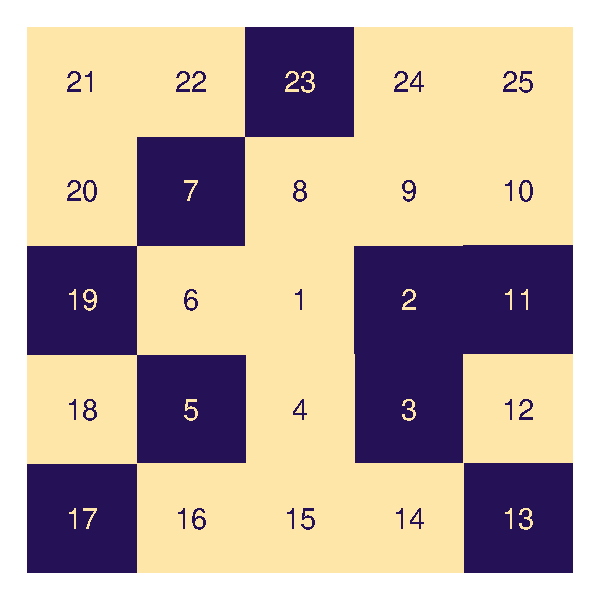
\includegraphics[width=0.8\linewidth]{figure/unnamed-chunk-2-1} \end{center}
\end{column}
\end{columns}
\end{frame}

\begin{frame}{Ulam's spiral}
\protect\hypertarget{ulams-spiral}{}
\begin{columns}[T]
\begin{column}{0.4\textwidth}
\begin{itemize}
\item
  Prominent diagonal, horizontal and vertical lines containing large
  number of primes.
\item
  Not unsurprising, as these correspond to certain prime-generating
  polynomials such as \(x^2 - x + 41\) (Euler's).
\item
  Nonetheless, connected to many unsolved areas of mathematics!

  \begin{itemize}
  \tightlist
  \item
    Riemann Hypothesis
  \item
    Goldbach's conjecture
  \item
    Twin prime conjecture
  \item
    Legendre's conjecture
  \end{itemize}
\end{itemize}
\end{column}

\begin{column}{0.6\textwidth}
\vspace{-2em}

\begin{center}
\includegraphics[height=0.9\textheight]{figure/unnamed-chunk-3-1} \end{center}
\end{column}
\end{columns}
\end{frame}

\begin{frame}{Does the density converge?}
\protect\hypertarget{does-the-density-converge}{}
As \(x\to\infty\), the prime density \(\pi(x)/x\) diminishes at a slow
rate. Reminiscent of an inverse logarithmic decrease!

\vspace{1em}

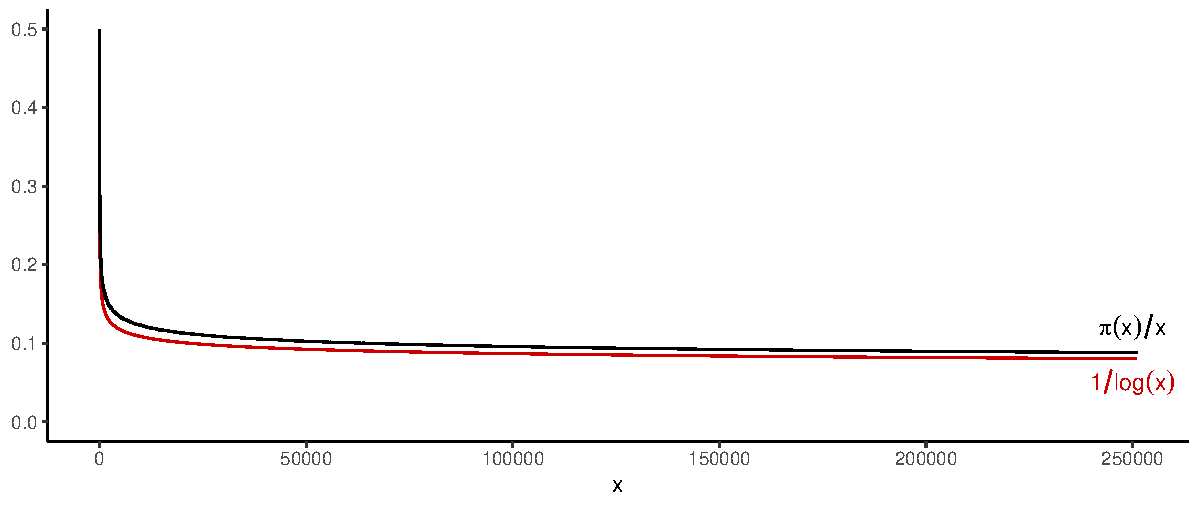
\includegraphics{figure/unnamed-chunk-4-1.pdf}
\end{frame}

\begin{frame}{The prime number theorem}
\protect\hypertarget{the-prime-number-theorem}{}
\begin{columns}[T]
\begin{column}{0.49\textwidth}
\begin{itemize}
\item
  The \emph{asymptotic} law of distribution of prime numbers states that
  \[
  \lim_{x\to\infty} \frac{\pi(x)/x}{1 / \log(x)} = \frac{\pi(x)}{x/\log(x)} = 1
  \] \pause
\item
  From this, we have \[
  \pi(x) \sim \frac{x}{\log(x)}
  \]
\item
  We now have an approximation for the prime counting function, which
  improves as \(x\) increases. In particular,
  \(\lim_{x\to\infty} x / \log (x) = \infty\).
\end{itemize}
\end{column}

\begin{column}{0.49\textwidth}
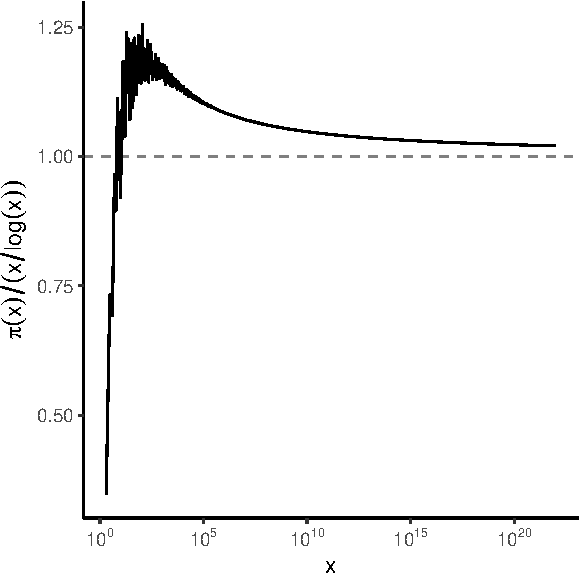
\includegraphics{figure/unnamed-chunk-5-1.pdf}
\end{column}
\end{columns}
\end{frame}

\begin{frame}{Using software}
\protect\hypertarget{using-software}{}
\usetikzlibrary{arrows}

\begin{center}
\huge
\begin{tikzpicture}[->,node distance=6cm,thick,main node/.style={circle,draw}]

  \node[] (1) {\color{navyblue}Mathematics};
  \node[] (4) [right of=1] {\color{solidpink}\texttt{Software}};
  

  \path[]
    (1.north) edge[bend left] node [above] {\textit{ideation}} (4.north)
    (4.south) edge[bend left] node [below] {\textit{results}} (1.south);
    
\end{tikzpicture}
\end{center}

Use software as a tool to\ldots{}

\begin{itemize}
\item
  Explore and visualise ideas
\item
  Confirm ideas numerically
\item
  Communicate results
\end{itemize}
\end{frame}

\begin{frame}[fragile]{Beyond this course}
\protect\hypertarget{beyond-this-course}{}
Static websites served on GitHub; 3-D plots and animation; Plotting GIS
shape files and maps; Reproducible research (\texttt{knitr}); Text
processing and analysis; Web and social media scraping; Creating
\texttt{R} packages; Web APIs; Parallel computing; Optimisation;
Mathematical and statistical modelling

\vspace{1em}

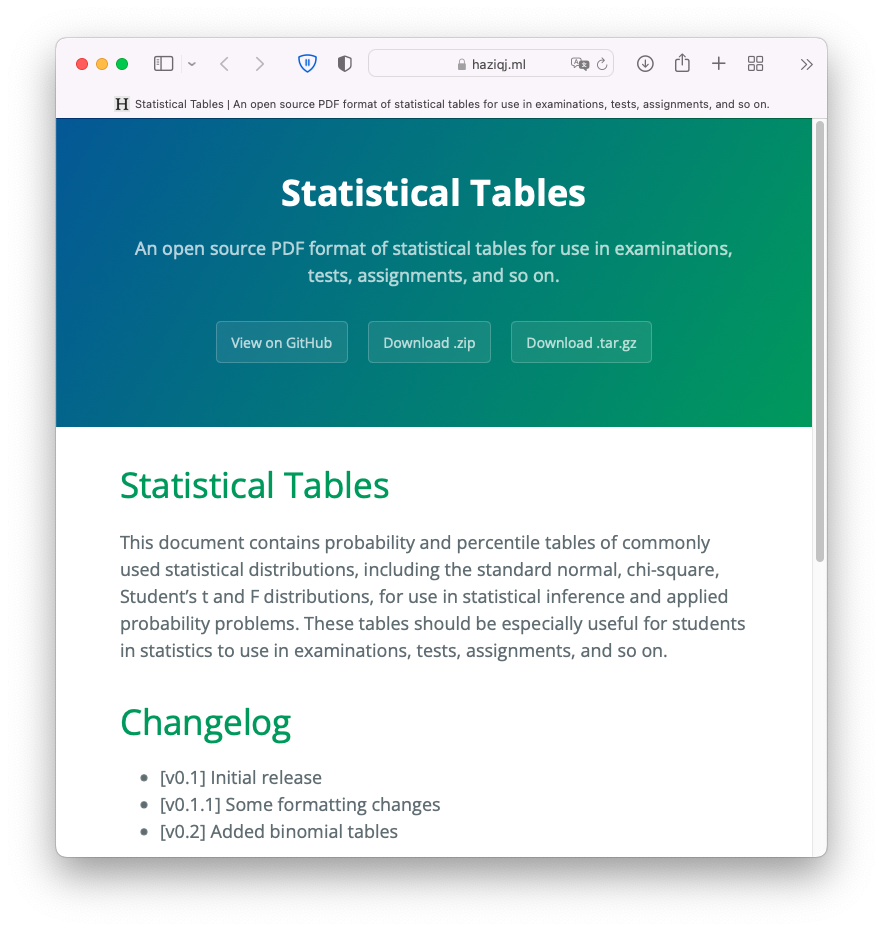
\includegraphics[width=0.31\linewidth]{figure/beyond1}
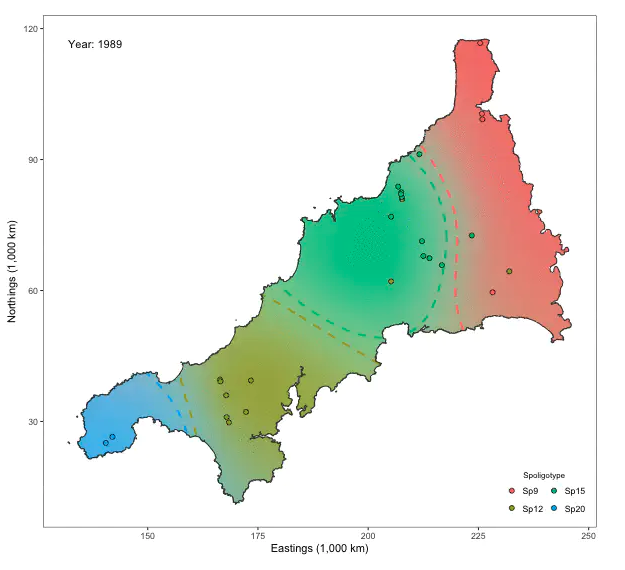
\includegraphics[width=0.31\linewidth]{figure/beyond2}
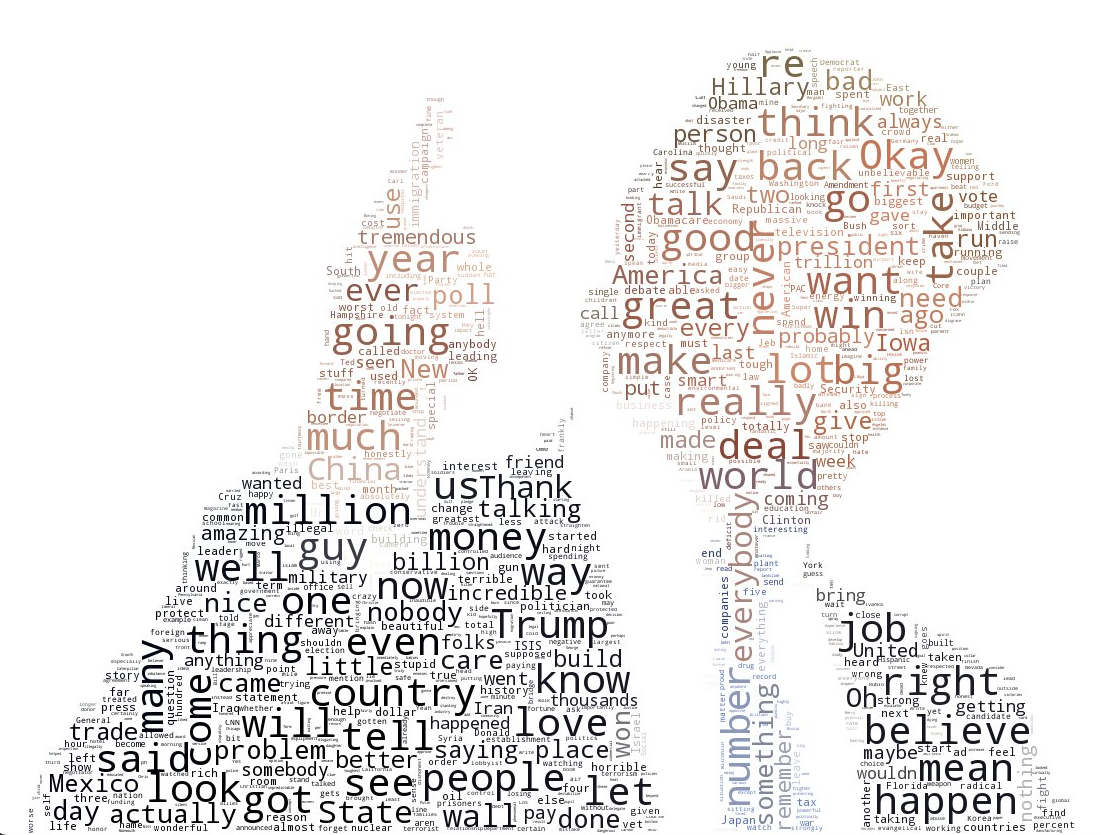
\includegraphics[width=0.31\linewidth]{figure/beyond3}
\end{frame}

\hypertarget{getting-started-1}{%
\section{Getting started}\label{getting-started-1}}

\hypertarget{instructions}{%
\subsection{Instructions}\label{instructions}}

\begin{frame}{Instructions}
\begin{alertblock}{IMPORTANT}
Check Canvas for detailed instructions regarding software installation
and sign up procedures.

\end{alertblock}

Important points:

\begin{itemize}
\item
  Use UBD e-mail in most cases to obtain Education Benefits
\item
  Pick a suitable username (one that you won't be embarassed to use in a
  few years time!)
\item
  Practice safe and secure passwords
\item
  When using Lab PCs, best to create a personal folder and keep all your
  work files in there.
\item
  Recommended to use USB drives (make sure they're clean!) or some cloud
  service (Dropbox, Sharepoint, Google Drive, etc.)
\end{itemize}
\end{frame}

\hypertarget{software-overview}{%
\subsection{Software overview}\label{software-overview}}

\begin{frame}[fragile]{Software overview}
\begin{enumerate}
\item
  MATLAB--more details in the upcoming slides.
\item
  RStudio Desktop

  \begin{itemize}
  \tightlist
  \item
    RStudio is installed on campus computers.
  \item
    It is free to install on your personal
    computers--\url{https://www.rstudio.com/products/rstudio/download/}
  \item
    You may also need to install the \texttt{R} language too, depending
    on your system. Do a Google search for `R Windows download' or
    similar.
  \end{itemize}
\item
  Git, github.com and GitHub Desktop

  \begin{itemize}
  \tightlist
  \item
    Please sign up for an account at github.com/signup using your UBD
    e-mail.
  \item
    You will be invited to join the course organization
    (\texttt{sm2302}) in due course.
  \item
    Assignments will be distributed and collected via GitHub.
  \end{itemize}
\item
  Overleaf.com

  \begin{itemize}
  \tightlist
  \item
    Please sign up for an account at
    \url{https://www.overleaf.com/register}
  \end{itemize}
\end{enumerate}
\end{frame}



\renewcommand{\bs}[1]{\boldsymbol{#1}}
\newcommand{\mb}[1]{\mathbf{#1}} 
\newcommand{\mc}[1]{\mathcal{#1}} 
\newcommand{\mbb}[1]{\mathbb{#1}} 
\newcommand{\txt}[1]{\texttt{#1}} 
\newcommand{\pdiff}[3]{ \if 1#1 
	\frac{\partial #2}{\partial #3} \else \frac{\partial^{#1} #2}{\partial 
		#3^{#1}}\fi}
\newcommand{\ppdiff}[3]{\frac{\partial^2 #1}{\partial #2 \partial #3}}
\newcommand{\sdiff}[3]{ \if 1#1 \frac{d #2}{d #3} \else \frac{d^{#1} #2}{d 
		#3^{#1}}\fi}
\newcommand{\e}{\mbox{e}}
\newcommand{\rvec}[1]{\overrightarrow{#1}}
\newcommand{\uvec}[3]{#1\,\mb{i}~ #2\,\mb{j}~ #3\,\mb{k}}

\subsection{MATLAB}
\begin{frame}{\txt{MATLAB}}
\begin{itemize}
	\item \txt{MATLAB} is a high-level language and interactive environment for numerical computation,
	visualization and programming.
	\begin{itemize}
		\item Analyze data
		\item Develop algorithms
		\item Create models and applications
	\end{itemize}
	\item We will reinforce some calculus concepts and its applications using \txt{MATLAB}, such as
	\begin{itemize}
		\item Numerical differentiation
		\item Numerical Integration
		\item Root-finding methods
	\end{itemize}
\end{itemize}
\end{frame}

\begin{frame}{Software}
\txt{MATLAB} is installed in the campus computer labs. 
However, if you wish to work from home or on your laptop, you can either
\begin{enumerate}
	\item use \txt{MATLAB} Online on your web browser; or
	\item install \txt{MATLAB} on your personal computer. 
\end{enumerate}

\begin{alertblock}{MATLAB Campus-wide suite}
To install or use \txt{MATLAB} on your web browser, you need to create a Mathworks
account using your UBD e-mail. You can access the UBD campus-wide suite using your mathworks account.\\
Please refer to the \txt{MATLAB} individual CWL installation guide document.
\end{alertblock}
\end{frame}

\begin{frame}{MATLAB Online}
\begin{center}
	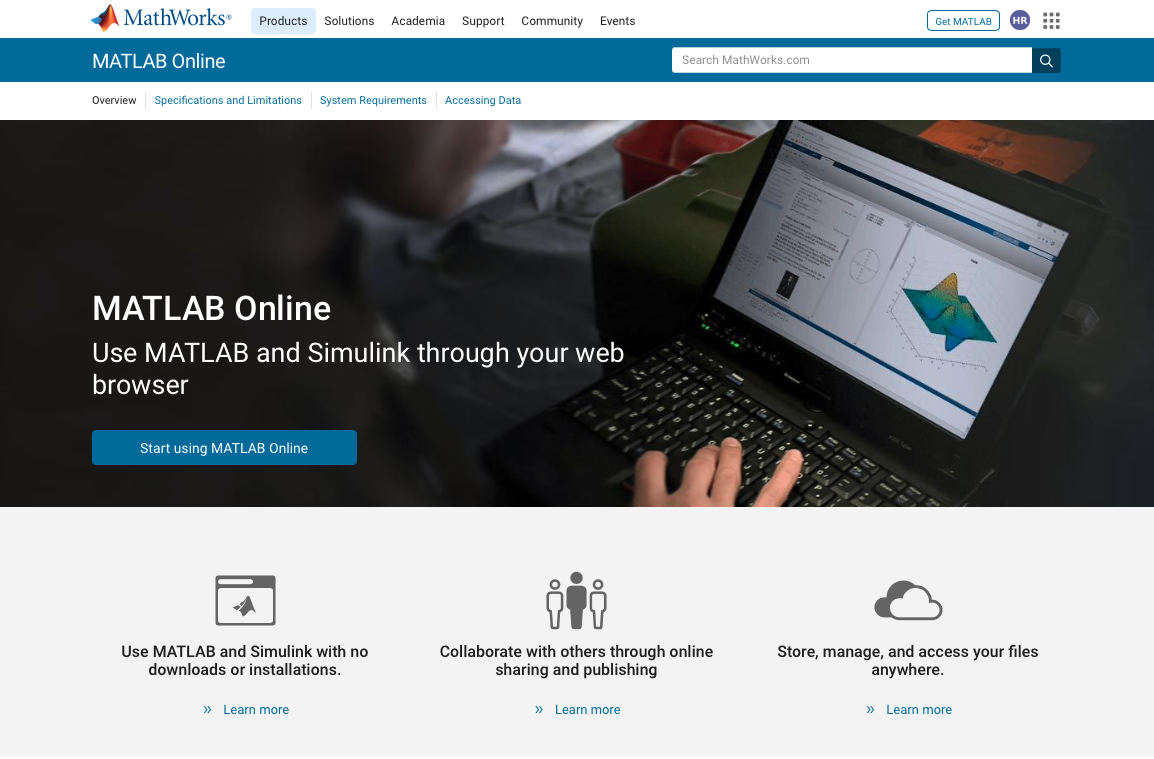
\includegraphics[width=0.6\textwidth]{matlab_online}
\end{center}
\url{https://matlab.mathworks.com}
\end{frame}



\begin{frame}{MATLAB Graphical Interface}
\begin{columns}
\begin{column}[T]{0.35\textwidth}
\begin{itemize}
	\item Command window
	\item Workspace
	\item Current folder
	\item Command history
	\item Editor
	\end{itemize}
\end{column}
\begin{column}[T]{0.75\textwidth}
	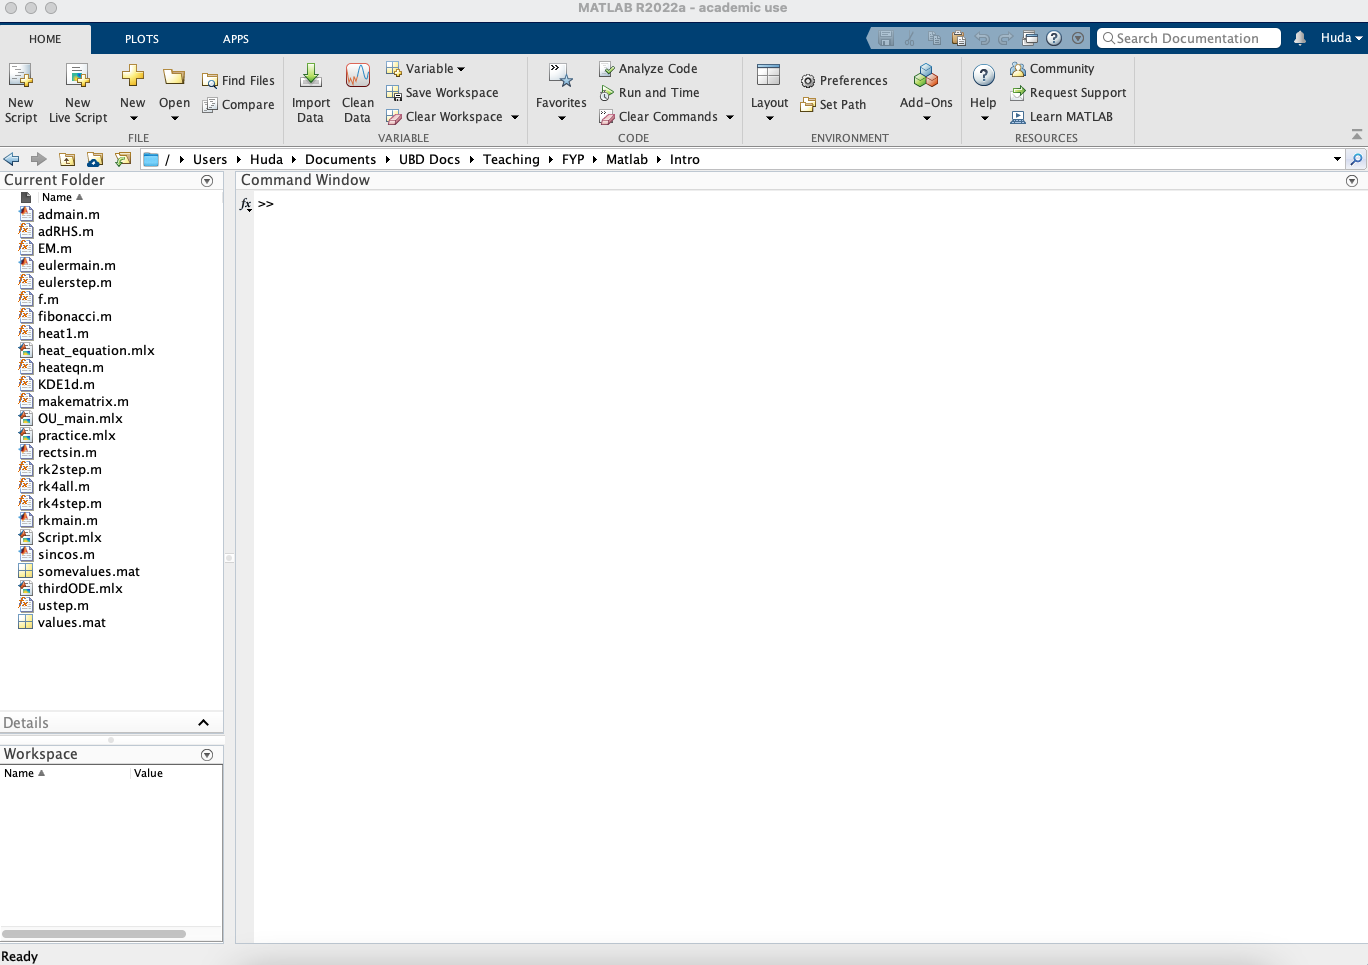
\includegraphics[width=0.85\textwidth]{initial_matlab}
\end{column}
\end{columns}

\end{frame}


\end{document}		
